\documentclass[11pt]{article}

\usepackage[margin=1in]{geometry}
\usepackage{graphicx}
\usepackage{booktabs}
\usepackage{multirow}
\usepackage{amsmath}
\usepackage{hyperref}
\usepackage[numbers]{natbib}
\usepackage{xcolor}

\title{Representation and Uncertainty in Action-Conditioned World Models:\\
A DINO-WM Course Project Study}
\author{Course Project Team}
\date{\today}

\begin{document}
\maketitle

\begin{abstract}
This project studies two controlled modifications to DINO-WM on PointMaze: replacing DINOv2 patch tokens with DINOv2 CLS tokens, and extending the deterministic latent transition model with a lightweight Gaussian predictor. We reproduced the pretrained PointMaze planning baseline, implemented the Gaussian transition head, and completed a formal \(3\)-seed \( \text{patch/CLS} \times \text{deterministic/Gaussian} \) matrix. We then added a larger-sample planning follow-up because the original \(n\_\text{evals}=3\) setting saturated the binary success metric. The resulting evidence shows that DINOv2 patch plus deterministic dynamics remains the strongest completed baseline, DINOv2 CLS plus deterministic dynamics is surprisingly competitive on PointMaze, and the Gaussian extension improves training losses without showing a stable planning benefit. Cross-environment pretrained sanity checks further indicate that the local setup generalizes to Wall and can succeed on PushT when the planning budget is made closer to the official configuration.
\end{abstract}

\section{Introduction}
World models aim to predict future states conditioned on actions and then use those predictions for planning. DINO-WM is a strong recent baseline because it combines frozen visual features from DINOv2, a latent transition model, and test-time model-predictive planning \citep{zhou2024dinowm}. Its central claim is that strong pretrained visual features can substantially improve downstream planning quality.

This project studies two questions while keeping the high-level pipeline fixed:
\[
\text{image encoder} \rightarrow \text{latent transition model} \rightarrow \text{planning}.
\]

The first is a \textbf{representation study}: how much does the latent visual representation matter for action-conditioned prediction and planning? The second is a \textbf{dynamics study}: can a lightweight stochastic extension improve the latent transition model compared with a purely deterministic predictor?

\section{Project Scope}
The original broader plan proposed comparing several representation families, including DINOv2 patch tokens, DINOv2 CLS, DINOv3, V-JEPA, DINO-Tok, and VFM-VAE. In practice, integrating multiple new foundation models turned out to be a separate engineering phase. For the completed experimental core, we therefore focused on a smaller but defensible matrix:

\begin{itemize}
\item DINOv2 patch tokens as the main baseline
\item DINOv2 CLS token as the key representation ablation
\item deterministic latent transition
\item Gaussian latent transition
\end{itemize}

This scope is sufficient to answer the two central project questions while keeping implementation and evaluation manageable.
Later encoder families are therefore treated as exploratory extensions rather than as part of the core completed study.

\section{Method}
\subsection{Baseline DINO-WM Pipeline}
The repository follows the standard DINO-WM structure:
\begin{itemize}
\item \textbf{Observation model}: a frozen DINOv2 encoder maps each image to latent features.
\item \textbf{Transition model}: a ViT-based dynamics model predicts the next latent state from past latent states and actions.
\item \textbf{Decoder}: an image decoder is optional and mainly used for visualization.
\item \textbf{Planner}: a CEM-style MPC planner searches action sequences in latent space.
\end{itemize}

\subsection{Representation Study}
We compare two encoders already supported by the repository:
\begin{itemize}
\item DINOv2 patch tokens \citep{oquab2023dinov2}
\item DINOv2 CLS token \citep{caron2021emerging}
\end{itemize}

The contrast is simple: patch tokens preserve spatial structure and local semantics, while CLS compresses the image into a single global token. Our initial hypothesis was that CLS would be weaker for control because it discards spatial detail that may matter for action-conditioned prediction.

\subsection{Dynamics Study}
The original deterministic model predicts
\[
(z_t, a_t) \rightarrow \hat z_{t+1}.
\]
We extend it to a Gaussian latent model:
\[
(z_t, a_t) \rightarrow (\mu_{t+1}, \log \sigma^2_{t+1}).
\]

Training uses Gaussian negative log-likelihood with a small MSE auxiliary term:
\begin{verbatim}
logvar = torch.clamp(logvar, -5, 5)
var = torch.exp(logvar)
gaussian_nll = ((target - mu) ** 2 / var + logvar).mean()
loss = gaussian_nll + 0.1 * mse(mu, target)
\end{verbatim}

For rollout and planning, we use \(\mu\) as the predicted latent state.

\section{Implementation Details}
\subsection{Environment}
The official repository targets Linux, so the experiments were run in WSL2 Ubuntu 24.04 with Python 3.9, MuJoCo 2.1, CUDA-enabled PyTorch, and the repository environment created from \texttt{environment.yaml}.

\subsection{Local Compatibility Fixes}
Several practical fixes were required before experiments could run end-to-end:
\begin{itemize}
\item WSL-specific Hydra configs replaced the default Slurm launcher.
\item MuJoCo 2.1 was installed manually for \texttt{mujoco\_py}.
\item DINOv2 loading was pinned to a Python-3.9-compatible ref.
\end{itemize}

The CLS ablation also exposed a structural limitation: the current decoder assumes a spatial patch grid, whereas CLS provides a single token. For this reason, CLS experiments were run with the decoder disabled, which is still valid because the decoder is optional in the original DINO-WM design.

\section{Experimental Setup}
\subsection{Main Environment}
The main controlled ablation study was performed on \texttt{PointMaze}. This environment is the simplest way to validate the full loop:
\[
\text{dataset} \rightarrow \text{training} \rightarrow \text{checkpoint} \rightarrow \text{planning}.
\]

\subsection{Matrix Configurations}
The core completed matrix is:
\begin{itemize}
\item patch + deterministic
\item CLS + deterministic
\item patch + Gaussian
\item CLS + Gaussian
\end{itemize}

We ran a \(3\)-seed formal matrix with:
\begin{itemize}
\item training epochs: \(3\)
\item rollout count: \(64\)
\item planning evaluations: \(n\_\text{evals}=3\)
\end{itemize}

\subsection{Larger-Sample Follow-Up}
Because \(n\_\text{evals}=3\) made \texttt{success\_rate} saturate at \(1.0\), we added a larger-sample planning follow-up. In principle this should have been direct \(n\_\text{evals}=10\) for all checkpoints, but WSL stability was uneven. The practical workaround was:
\begin{itemize}
\item direct \(n\_\text{evals}=10\) where stable
\item otherwise two \(n\_\text{evals}=5\) shards whose results were combined for reporting
\end{itemize}

\section{Results}
\subsection{Formal Three-Seed Matrix}
Table~\ref{tab:formal} summarizes the core formal matrix.
Unless stated otherwise, the paper's main comparative conclusions are drawn from this formal matrix and its associated planning metric.

\begin{table}[h]
\centering
\caption{Three-seed PointMaze formal matrix.}
\label{tab:formal}
\begin{tabular}{llccc}
\toprule
Encoder & Transition & Mean train loss & Mean val loss & Mean state distance \\
\midrule
DINOv2 patch & deterministic & 0.0825 & 0.0429 & 3.2806 \\
DINOv2 CLS & deterministic & 0.0411 & 0.0240 & 3.3047 \\
DINOv2 patch & Gaussian & -2.9815 & -3.1785 & 3.7772 \\
DINOv2 CLS & Gaussian & -3.0751 & -3.2282 & 3.3277 \\
\bottomrule
\end{tabular}
\end{table}

Figure~\ref{fig:formal-summary} visualizes the same formal matrix from two angles: planning quality and training objective.

\begin{figure}[h]
\centering
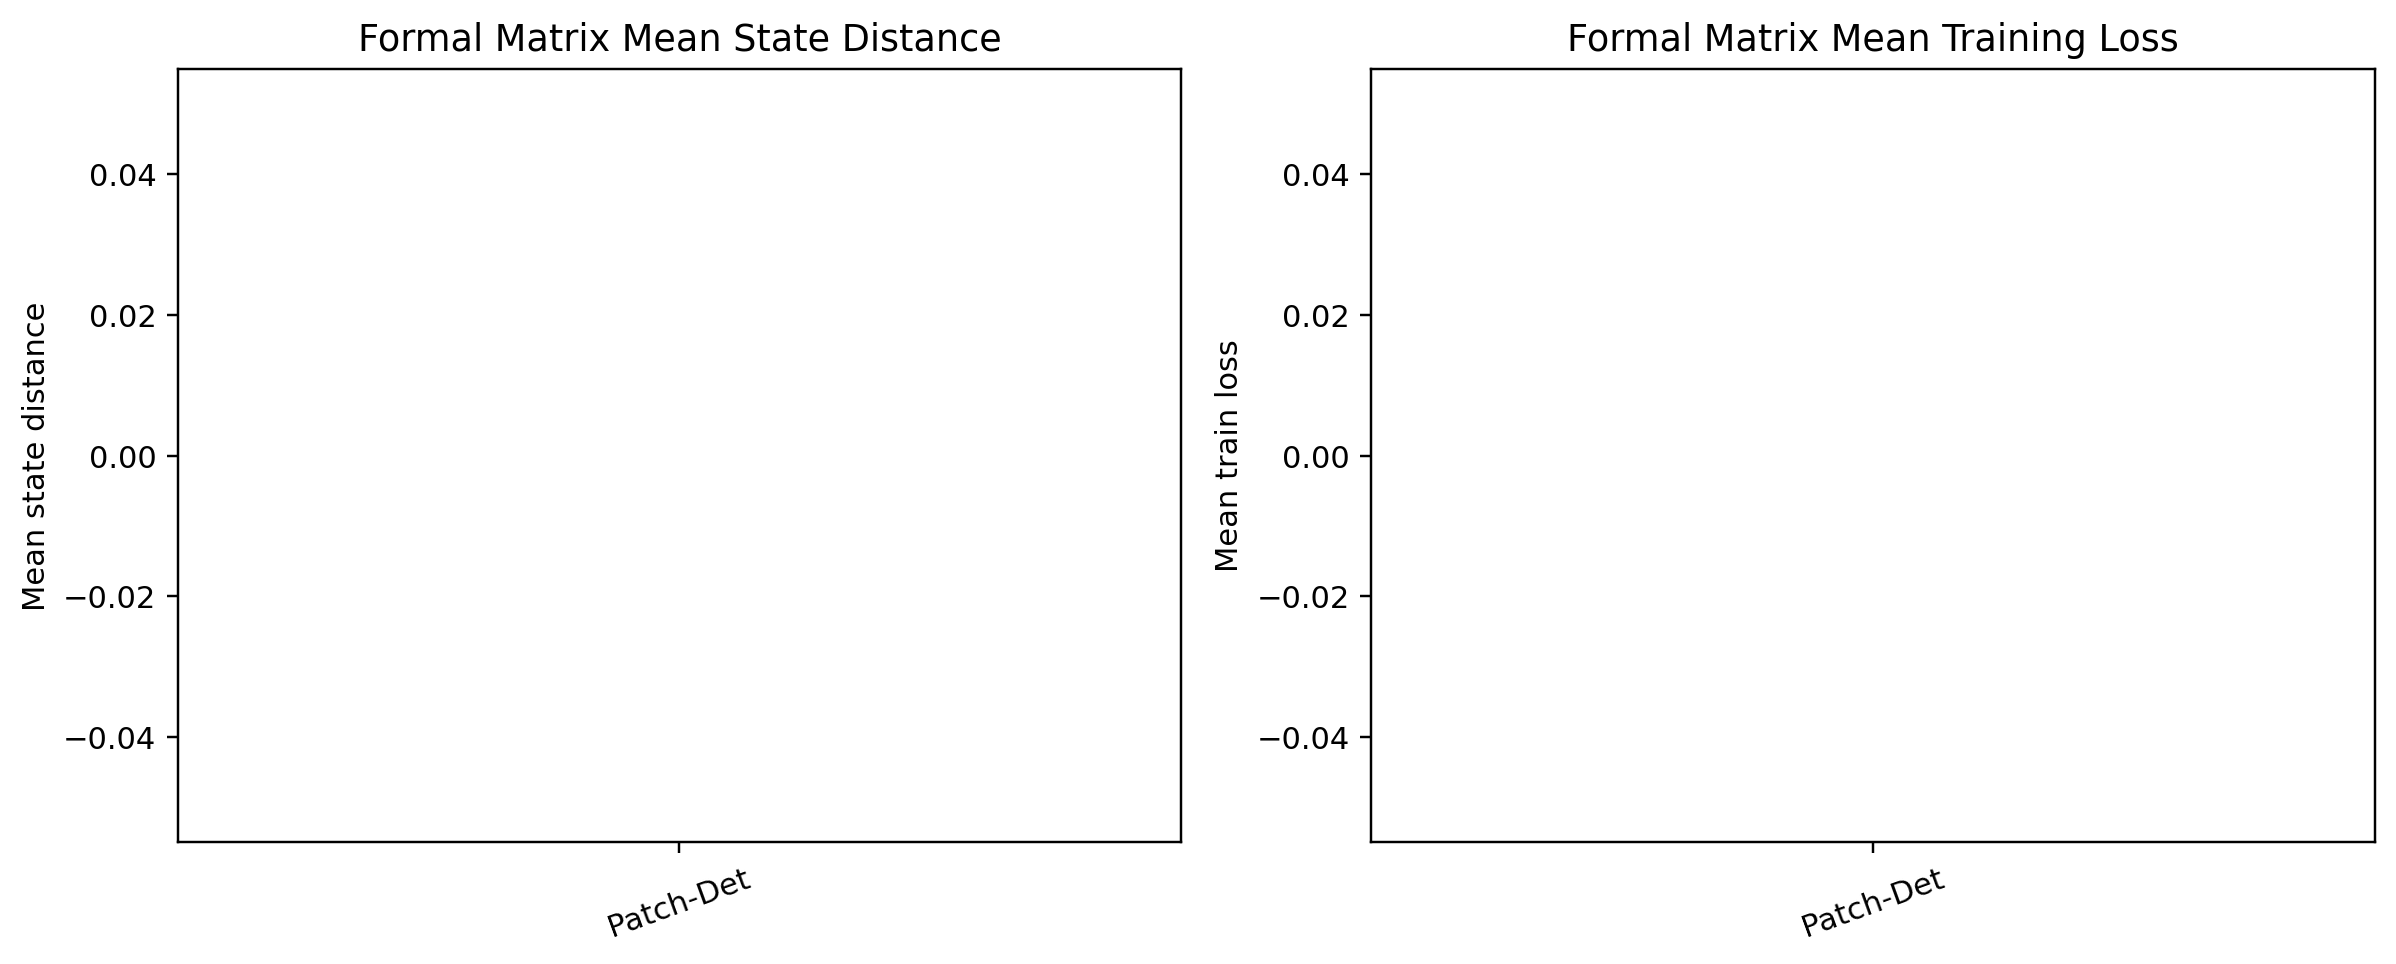
\includegraphics[width=0.95\linewidth]{figure/formal_matrix_summary.png}
\caption{Formal PointMaze matrix summary. Left: mean final state distance across the three-seed matrix. Right: mean training loss across the same matrix. The planning ranking does not mirror the Gaussian training objective advantage.}
\label{fig:formal-summary}
\end{figure}

The formal matrix supports three main conclusions:
\begin{itemize}
\item DINOv2 patch plus deterministic dynamics remains the strongest overall baseline.
\item DINOv2 CLS plus deterministic dynamics is much closer to patch than initially expected.
\item The Gaussian extension improves likelihood-style training losses, but this does not translate into a stable planning advantage.
\end{itemize}

\subsection{Larger-Sample PointMaze Follow-Up}
Table~\ref{tab:largeeval} summarizes the cleanest larger-sample closeout view.

\begin{table}[h]
\centering
\caption{PointMaze larger-sample follow-up summary.}
\label{tab:largeeval}
\begin{tabular}{lll}
\toprule
Group & Coverage & Aggregate picture \\
\midrule
Seed-0 patch deterministic & complete & \(3.1738\) \\
Seed-0 CLS deterministic & complete & \(\sim 3.5291\) \\
Seed-0 patch Gaussian & complete & \(\sim 4.3382\) \\
Seed-0 CLS Gaussian & complete & \(\sim 3.8242\) \\
Seed-1 patch deterministic & complete & \(\sim 4.1189\) \\
Seed-1 CLS deterministic & partial & shard B only, \(3.9672\) \\
Seed-1 patch Gaussian & complete & \(\sim 3.9366\) \\
Seed-1 CLS Gaussian & complete & \(\sim 3.9565\) \\
Seed-2 patch deterministic & complete & \(\sim 3.4584\) \\
Seed-2 CLS deterministic & incomplete & not included in final comparison \\
Seed-2 patch Gaussian & complete & \(\sim 4.3641\) \\
Seed-2 CLS Gaussian & incomplete & not included in final comparison \\
\bottomrule
\end{tabular}
\end{table}

Figure~\ref{fig:patch-large} shows the patch branch only, because that branch reached the cleanest multi-seed larger-sample coverage.

\begin{figure}[h]
\centering
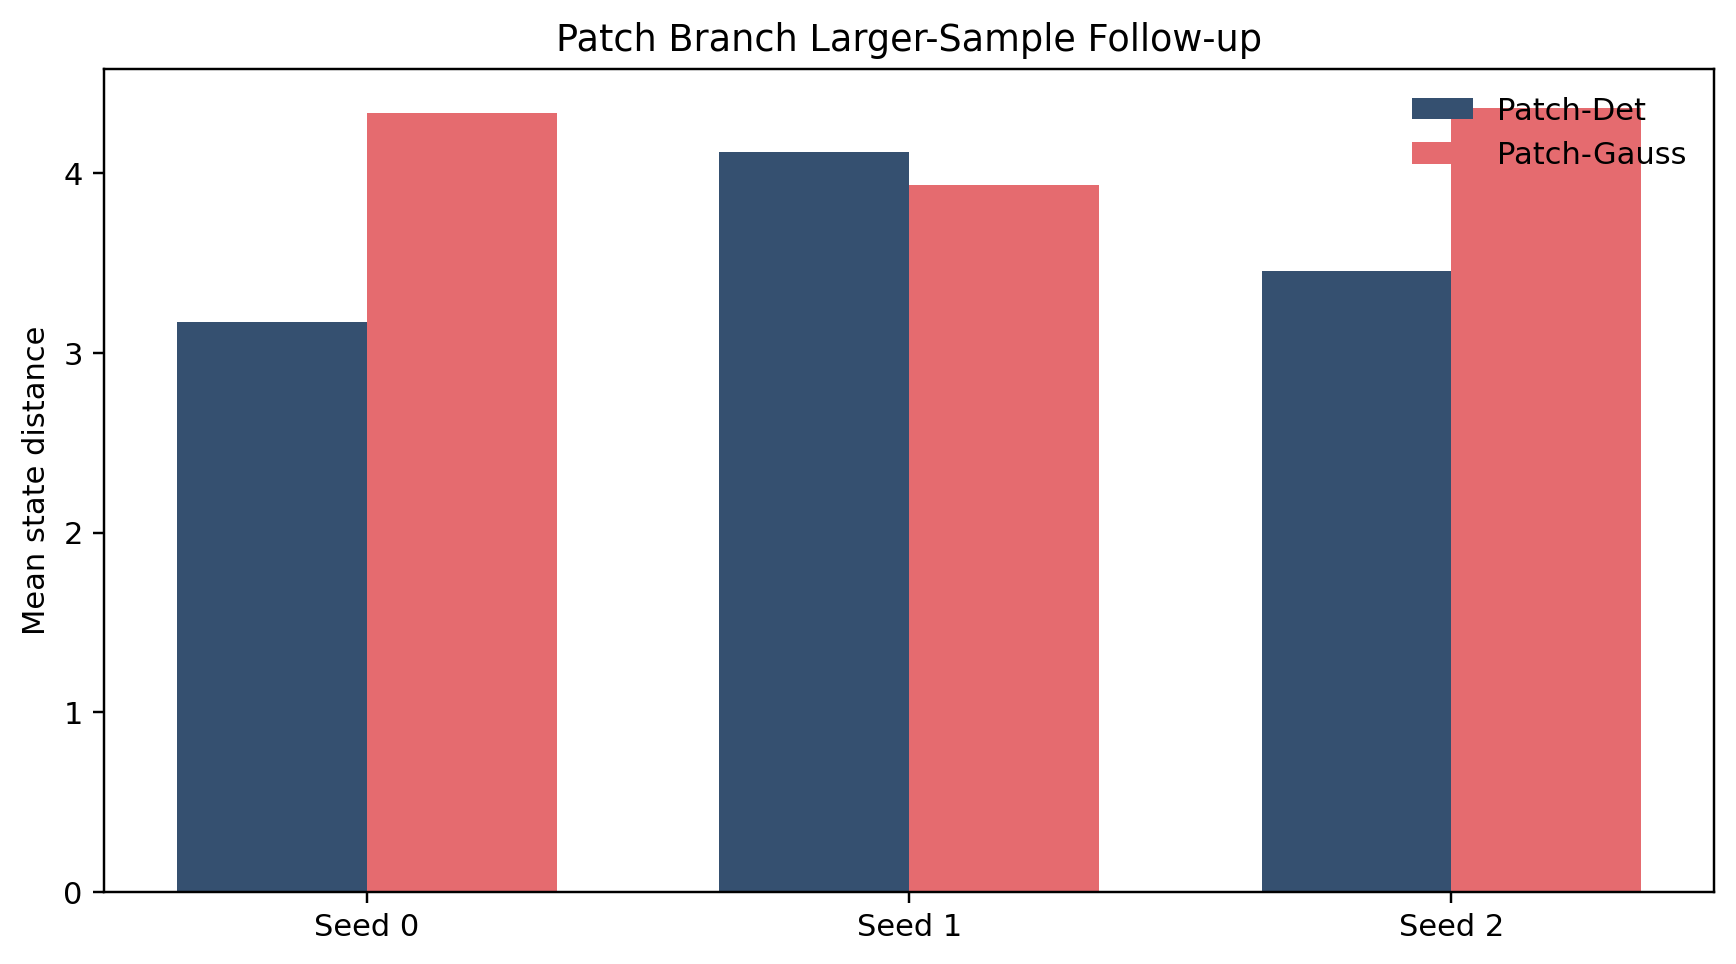
\includegraphics[width=0.78\linewidth]{figure/patch_large_eval.png}
\caption{Patch branch larger-sample follow-up. Deterministic patch remains the strongest patch-side baseline across the completed seed groups.}
\label{fig:patch-large}
\end{figure}

These larger-sample results strengthen the formal-matrix interpretation:
\begin{itemize}
\item deterministic patch remains the most reliable patch-side baseline
\item Gaussian patch does not show a consistent planning benefit
\item CLS remains competitive, but its larger-sample evidence is only partial
\end{itemize}

For the final paper, we treat the completed larger-sample runs as supportive evidence rather than as a second perfectly symmetric benchmark. The patch branch is the cleanest completed follow-up, while the CLS branch should be read as partial corroboration only.

\subsection{Why \texttt{success\_rate} Was Not Enough}
At first, repeated \texttt{success\_rate = 1.0} results looked like a pure sample-size problem. That was correct, but only partially complete. After increasing evaluation coverage, a second issue became clear:
\begin{itemize}
\item \texttt{success\_rate} often remained saturated
\item \texttt{mean\_state\_dist} still showed meaningful variation
\end{itemize}

This means the evaluation problem has two layers:
\begin{enumerate}
\item small \(n\_\text{evals}\) makes the binary success metric statistically weak
\item even with larger sample size, the PointMaze success metric is still too coarse
\end{enumerate}

Therefore, the most defensible reporting strategy is to use \texttt{mean\_state\_dist} as the primary planning metric and treat \texttt{success\_rate} only as a coarse indicator.

\subsection{Cross-Environment Pretrained Sanity}
To test whether the local planning stack generalized beyond PointMaze, we also ran pretrained planning sanity checks on Wall and PushT. The completed runs are summarized in Figure~\ref{fig:crossenv}.
These runs are best interpreted as feasibility checks for the local planning stack, not as a second controlled benchmark comparable to the PointMaze ablation matrix.

\begin{figure}[h]
\centering
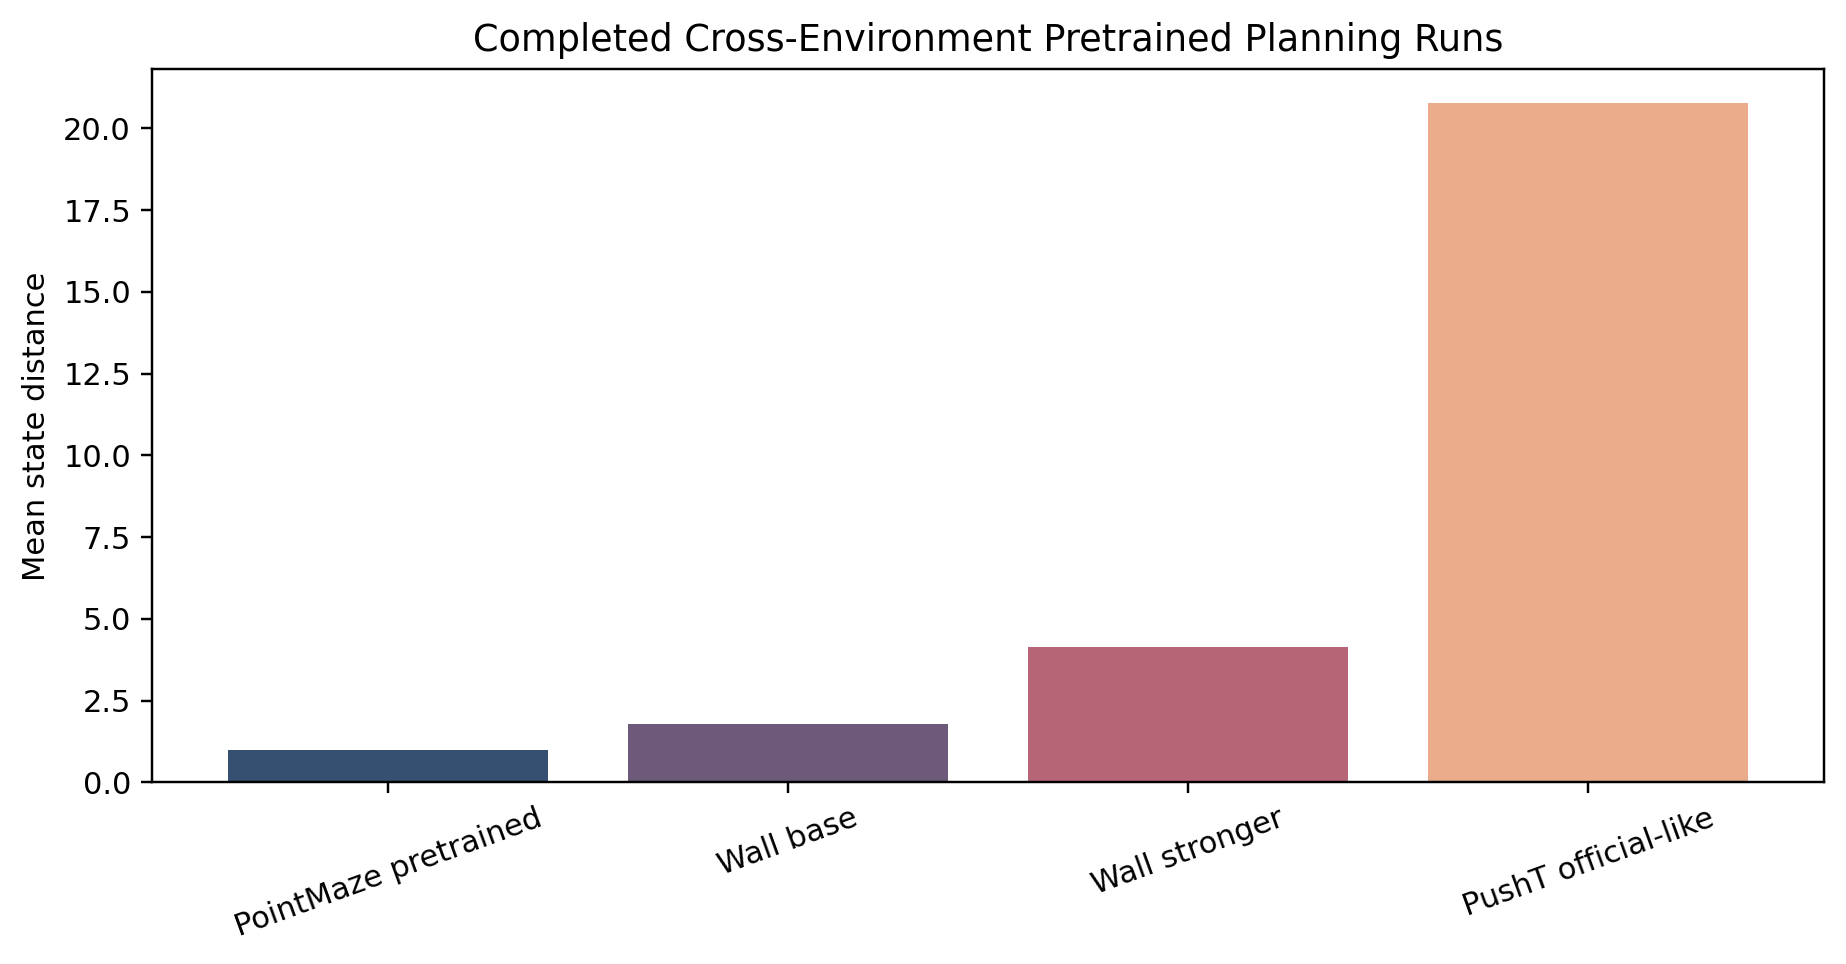
\includegraphics[width=0.82\linewidth]{figure/cross_env_sanity.png}
\caption{Completed cross-environment pretrained planning runs. Reduced- and medium-budget PushT runs are not plotted because they stalled before \texttt{final\_eval}.}
\label{fig:crossenv}
\end{figure}

The qualitative interpretation is:
\begin{itemize}
\item Wall passes cleanly under both a light local budget and a stronger local budget.
\item PushT fails under an aggressively reduced budget.
\item PushT improves under a medium budget but still stalls.
\item PushT succeeds once the planning budget is made much closer to the official configuration.
\end{itemize}

This is useful because it shows that the earlier PushT failures were primarily caused by underpowered planning budgets, not by a fundamentally broken local setup.

\section{Discussion}
The project now has runnable implementations for both requested axes:
\begin{itemize}
\item \textbf{representation}: patch tokens vs.\ CLS
\item \textbf{dynamics}: deterministic vs.\ Gaussian
\end{itemize}

The current evidence supports a narrower conclusion than the original hypothesis. We expected patch structure to clearly dominate CLS. Instead, CLS remained competitive on PointMaze. At the same time, the Gaussian extension improved training losses more than it improved planning quality. This outcome reinforces the value of a controlled ablation setup: even modest architectural changes can produce results that differ from the initial intuition.

One plausible explanation is that the Gaussian objective helps local next-step fitting more than downstream multi-step planning. In other words, better likelihood-style training losses do not necessarily imply better rollout behavior under MPC, especially when planning quality depends on compounding prediction errors rather than on one-step reconstruction accuracy alone.

\subsection{What Has Not Been Demonstrated Yet}
This is still not a full benchmark study. The main controlled evidence is still PointMaze-centric, and the larger-sample CLS branch is incomplete. Additional encoder families such as DINOv3 and V-JEPA were explored as follow-on work, but they are not part of the completed matrix used for the paper's main conclusions.

\subsection{Encoder-3 and Encoder-4 Status}
The next two encoder branches were scoped as:
\begin{itemize}
\item encoder 3: DINOv3 patch
\item encoder 4: V-JEPA
\end{itemize}

Their feasibility status is already informative:
\begin{itemize}
\item DINOv3 is currently blocked by Python \(3.9\) compatibility in the validated local environment.
\item V-JEPA progressed much further: an encoder-only wrapper was implemented locally, pretrained visual-encoder weights were shown to load successfully, and a PointMaze training run completed its first three epochs with losses decreasing from \(0.2267/0.1116\) to \(0.1117/0.0957\) and then \(0.1002/0.0867\) for train/validation respectively.
\item This exploratory run is encouraging because it suggests that the local V-JEPA integration is trainable rather than merely loadable.
\item Even so, V-JEPA remains outside the completed paper matrix because its long-run training closeout and planning evaluation were still ongoing at the time of writing.
\end{itemize}

\section{Limitations}
\begin{itemize}
\item The main controlled study is still PointMaze-centric.
\item CLS uses no decoder, so decoder-side comparisons are unavailable.
\item The larger-sample follow-up is intentionally asymmetric: the patch branch is much cleaner than the CLS branch, so the paper treats it as supporting evidence rather than as a second formal matrix.
\item Even after the larger-sample follow-up, \texttt{success\_rate} remains partially saturated on PointMaze.
\item DINOv3 and V-JEPA were not part of the completed experimental matrix, so the paper does not make comparative claims about them.
\end{itemize}

\section{Conclusion}
This project turned the original DINO-WM course-project idea into a working experimental study. We reproduced the pretrained PointMaze baseline, ran a complete three-seed \( \text{patch/CLS} \times \text{deterministic/Gaussian} \) matrix, and added a larger-sample planning follow-up that made the final comparison more defensible.

The final practical conclusions are:
\begin{itemize}
\item DINOv2 patch plus deterministic dynamics remains the most reliable completed baseline.
\item DINOv2 CLS plus deterministic dynamics is more competitive than originally expected on PointMaze.
\item The Gaussian extension improves training losses but does not show a stable planning advantage.
\item Wall pretrained planning succeeds under the local setup.
\item PushT becomes viable only when the planning budget is much closer to the official configuration.
\end{itemize}

Exploratory follow-on work also indicates that the project infrastructure can support additional encoders beyond the completed matrix, although those extensions are not yet mature enough to change the paper's central conclusions.

The most important methodological lesson is that evaluation quality matters as much as model design. Increasing \(n\_\text{evals}\) was necessary, but it did not fully solve metric saturation. As a result, \texttt{mean\_state\_dist} provides the strongest basis for the project's final representation and dynamics conclusions.

\bibliographystyle{plainnat}
\bibliography{references}

\end{document}
